\chapter{Análisis de las imágenes \label{chap:Analisis}}

%%%%%%%%%%%%%%%%%%%%%%%%%%%%%%%%%%%%%%%%%%%%%%%%%%%%%%%%%%%%%%%%%%
\section{Procesado de datos y obtención de imágenes \label{sec:ProcesadoDatos}}
\noindent Los datos obtenidos durante el proceso de medición se almacenan en un tipo de imagen de formato \verb|.fits|. Cada píxel de esa imagen representa la carga en el nodo de sensado. Debido a que el \textit{Skipper}-CCD permite realizar la medición de carga de un píxel tantas veces como se desee, si se eligió tomar un número $N$ de muestreos por cada píxel del sensor, entonces la imagen \verb|.fits| producida tendrá $N$ píxeles por cada píxel real del sensor. Por ejemplo, si el sensor estuviera conformado por $16$ píxeles, $4$ filas y $4$ columnas y el número de muestreos elegido fuera de $3$, la imagen resultante tendría una dimensión de $4$ filas por $12$ columnas, como se ve en la Figura \ref{fig:Skipper2root_esquema}. Por esta razón, resulta necesario procesar la imagen generada, promediando los $N$ muestreos por píxel y así obtener una lectura de carga con muy bajo ruido a la vez de disminuir drásticamente el tamaño y peso de la imagen.

El procesamiento de las imágenes es llevado a cabo por el programa \verb|skipper2root.exe|, el cual genera una nueva imagen de formato \verb|.fits|, ya promediada y con el tamaño correspondiente a la cantidad total de píxeles del sensor que se utilizaron en la medición. A su vez, es este programa el que se encarga de restar la linea de base, utilizando las columnas del \textit{over-scan}, de forma de establecer el valor nulo de carga para cada fila del sensor.
\begin{figure}[h]
    \centering
    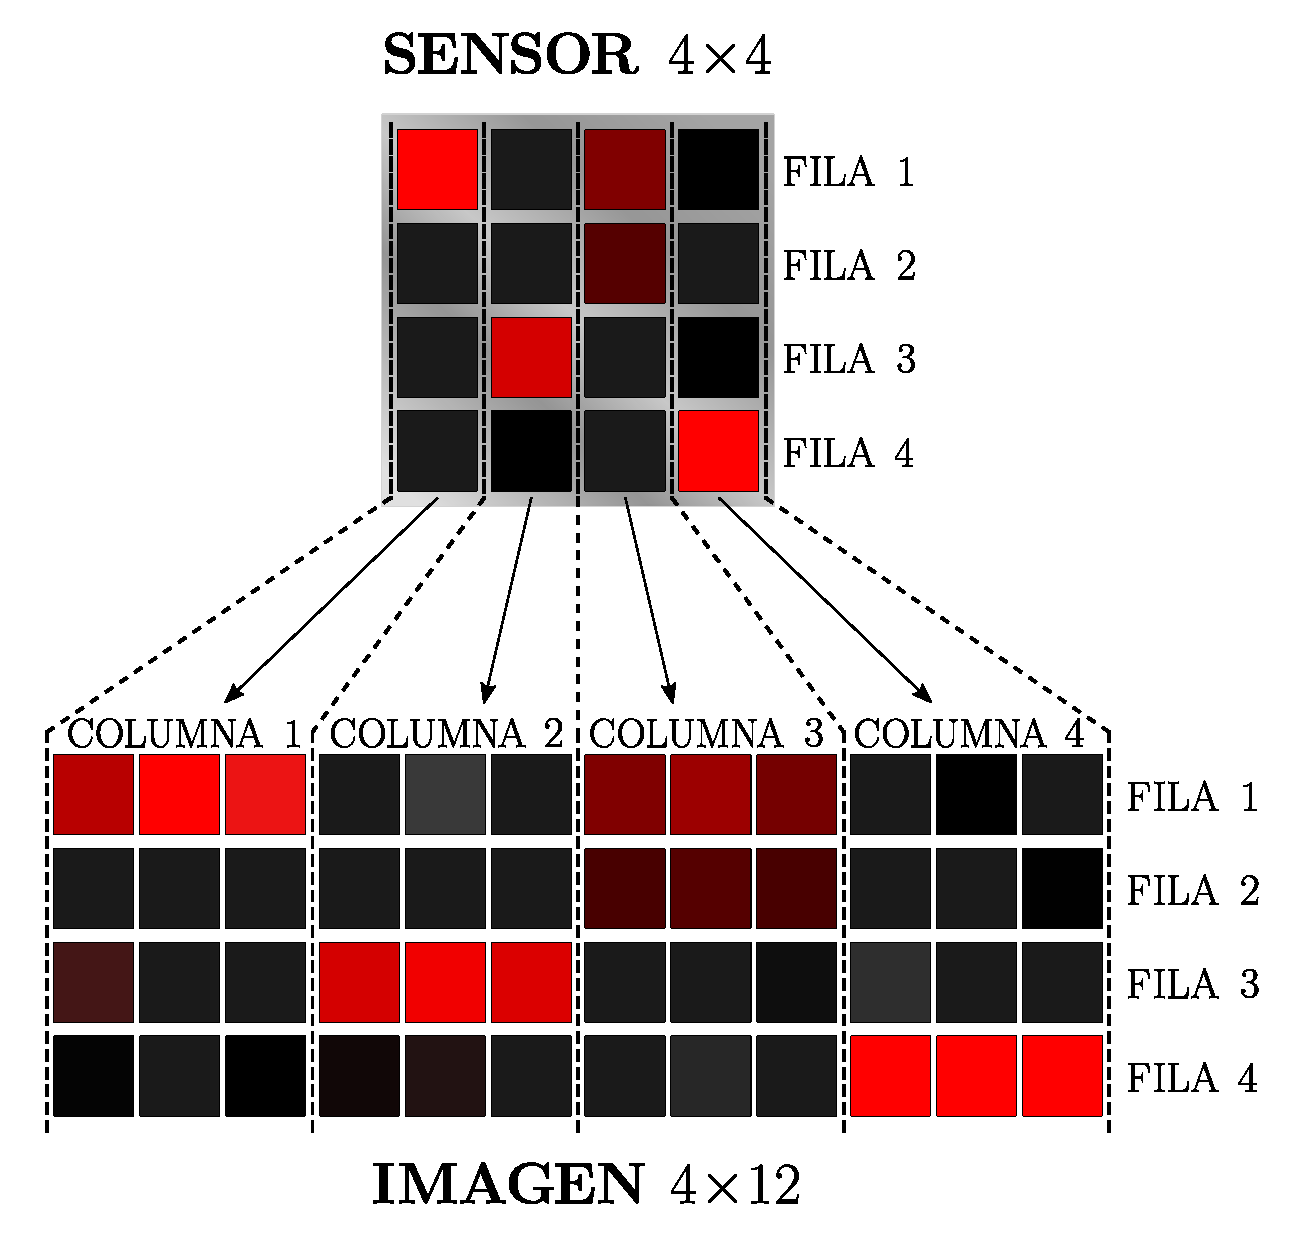
\includegraphics[scale=0.4]{Figs/skipper2root_scheme.pdf}
    \caption{\footnotesize{Ejemplo de la imagen resultante de medir con un sensor de $4\times4$ píxeles utilizando un muestreo de $3$ lecturas por píxel. La imagen resultante es de $4\times 12$ píxeles.}}
    \label{fig:Skipper2root_esquema}
\end{figure}
Estas nuevas imágenes tienen la información de la carga de los eventos medidos en cada píxel con muy bajo ruido gracias al muestreo utilizado. Sin embargo, los datos en ellas aún están en unidades analógico-digitales (ADUs), con lo cual, para estudiarlas en términos de la cantidad de carga es necesario utilizar una calibración ADU-electrones, que se obtenía con el método descripto en la Sección \ref{sec:Antecedentes}. Esta calibración está modelada por un polinomio de orden $4$ de la forma
\begin{equation*}
    e^{-} 
    = \alpha \mbox{ADU} 
    + \beta \mbox{ADU}^{2}
    + \gamma \mbox{ADU}^{3}
    + \delta \mbox{ADU}^{4}
\end{equation*}
y es diferente para cada de los cuadrantes del sensor.

Además, es necesario poder reconocer los conjuntos de píxeles contiguos con carga que pertenecen a un único evento. Con este fin, se utiliza otro programa, el cual hace uso de la calibración para transformar de ADUs a electrones además de reconocer los conjuntos de píxeles con carga por medio de un algoritmo de clusterización. Este programa se llama \verb|skeExtract.exe| y procesa todas las imágenes que \verb|skipper2root.exe| generó para así formar un nuevo tipo de archivo, de formato \verb|.root|, con toda la información de los eventos encontrados en las imágenes. A partir de este último, se realizan los análisis estadísticos utilizando \verb|C++| y las librerías para análisis de datos científicos desarrolladas por el CERN llamadas \textit{ROOT}.

Finalmente, un último código es utilizado, donde se implementan los cortes de calidad que filtran los eventos no deseados y dejan los que se deseen estudiar, para la construcción de los histogramas de carga. A partir de estos se realizan los ajustes y se obtienen los parámetros de interés, como el factor de Fano, la energía de creación electrón hueco y el espesor de la zona de colección parcial de carga.

%%%%%%%%%%%%%%%%%%%%%%%%%%%%%%%%%%%%%%%%%%%%%%%%%%%%%%%%%%%%%%%%%%
\section{Análisis y factibilidad}
\noindent En este trabajo se propone realizar un análisis profundo de las mediciones existentes, aplicando un corte de calidad a las imágenes que aumenta la detección de eventos, para así mejorar la estadística y la resolución con la que se calculan tanto el factor de Fano como la energía de creación electrón-hueco. %Sin embargo, aplicar este corte de calidad trae aparejado un sesgo en el conteo de carga de cada evento, tanto por defecto como por exceso, con lo cual es un efecto que debe corregirse.
En este sentido, es de gran importancia cuantificar el aumento en la estadística al modificar los parámetros usados en el programa de reconocimiento de clusters (\verb|skeExtract.exe|) y así poder establecer la factibilidad de la mejora en el cálculo de las incertezas de los valores antes mencionados.

El parámetro clave en este caso se llama \verb|EPIX| y es un valor umbral que define a partir de qué cantidad de carga se cuenta o no como un píxel vacío. Por ejemplo, para \verb|EPIX = 0.5|, todos los píxeles con carga menor o igual a $0.5$ se cuentan como píxeles vacíos, y los que tengan carga mayor a $0.5$ serán contabilizados normalmente, para \verb|EPIX = 1.5|, todos los píxeles con carga menor o igual a $1.5$ se cuentan como píxeles vacíos y los píxeles con carga mayor a $1.5$ se cuentan normalmente. En la Figura \ref{fig:HistogramaEPIX} puede verse un esquema de un histograma de los niveles de carga y cómo se sitúa el umbral \verb|EPIX| para contar la carga.
\begin{figure}[h]
%Como reproducir este gráfico: correr el script NivelesOcupacionCargaEPIX_e.py ubicado en /Escritorio/Tesis2021/Figs/pys_para_plots y buscar la imagen en /home/igna/Escritorio/Tesis2021/Figs/
    \centering
        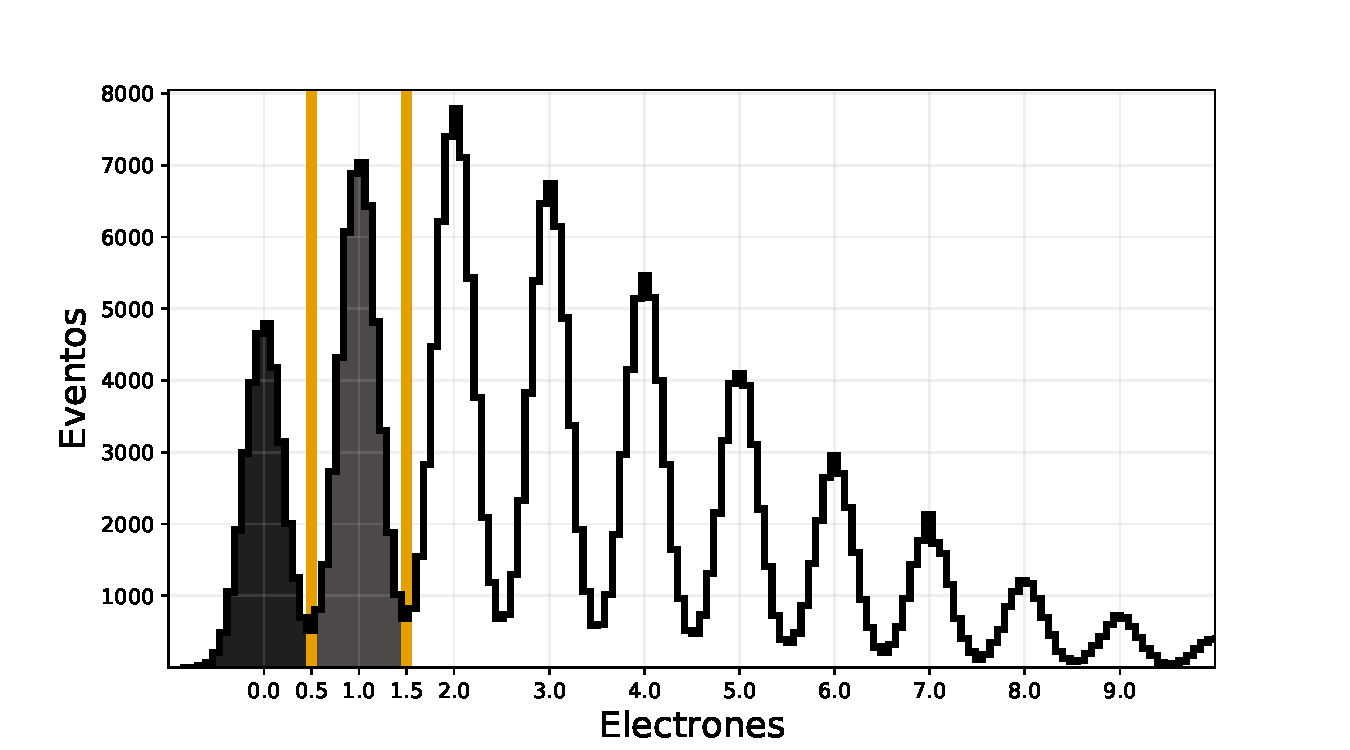
\includegraphics[scale=0.5]{Figs/EsquemaEPIX_histocarga.pdf}
    \caption{\footnotesize{Histograma de los datos obtenidos al iluminar el CCD con LED, correspondiente a una región con poca ocupación, donde se han marcado con dos rectas verticales los umbrales para \texttt{EPIX}$=0.5$ y $1.5$. Depende de cuál umbral sea usado, toda la carga que se encuentra a la izquierda del umbral se considera nula.}}
    \label{fig:HistogramaEPIX}
\end{figure}
En trabajos previos\cite{TesisKevin}, los valores obtenidos para el factor de Fano y energía de creación electrón-hueco, fueron calculados con un valor de \verb|EPIX = 0.5|. Se espera que al modificar este parámetro, el conteo de eventos varíe y que, en particular, aumente cuando el \verb|EPIX| aumenta. Esto se debe a que es muy común que se tenga un evento de interés, por ejemplo un cluster de $4$ píxeles de área y con una carga total de $180$ electrones (para el caso del flúor), y alrededor de este se acumulen píxeles con fondo, de por ejemplo $1$ o muy raramente $2$ electrones. En estos casos podría suceder que la conexión entre el cluster de interés y los píxeles con carga espuria se extiendan lo suficiente como para que el algoritmo reconozca un gran cluster con exceso de carga y sea desechado por el programa dado que no cumple con los cortes de calidad impuestos. También podría suceder que estos píxeles con carga espuria conecten $2$ clusters de interés, lo cual es un caso más extremo, dado que el algoritmo reconocería un único cluster de $\sim 360$ electrones, de forma que se perderían, no uno, sino dos eventos que podrían aportar positivamente a la estadística. Al aplicar un umbral que elimine los píxeles con carga espuria que se amontonan y/o conectan con clusters, el programa es capaz de diferenciar y contar los eventos correctamente.

En la Figura \ref{fig:ClusterPegoteado} se muestra un ejemplo de un evento de $179$ electrones para una medición con flúor, que es un evento de interés que el programa debería reconocer, y que hasta que no se eliminan los eventos de un electrón de la imagen, el programa lo identifica como un gran cluster con aproximadamente $40$ electrones más de carga y sin una forma definida (imagen central, píxeles pintados de blanco). A la derecha la imagen con el cluster individualizado y reconocido correctamente por el algoritmo al eliminar la carga excedente.
\begin{figure}[H]
%Para modificar este plot hay que ir a Escritorio/Tesis2021/Figs/pys_para_plots y modificar clusters_no_pegoteados.py
    \centering
    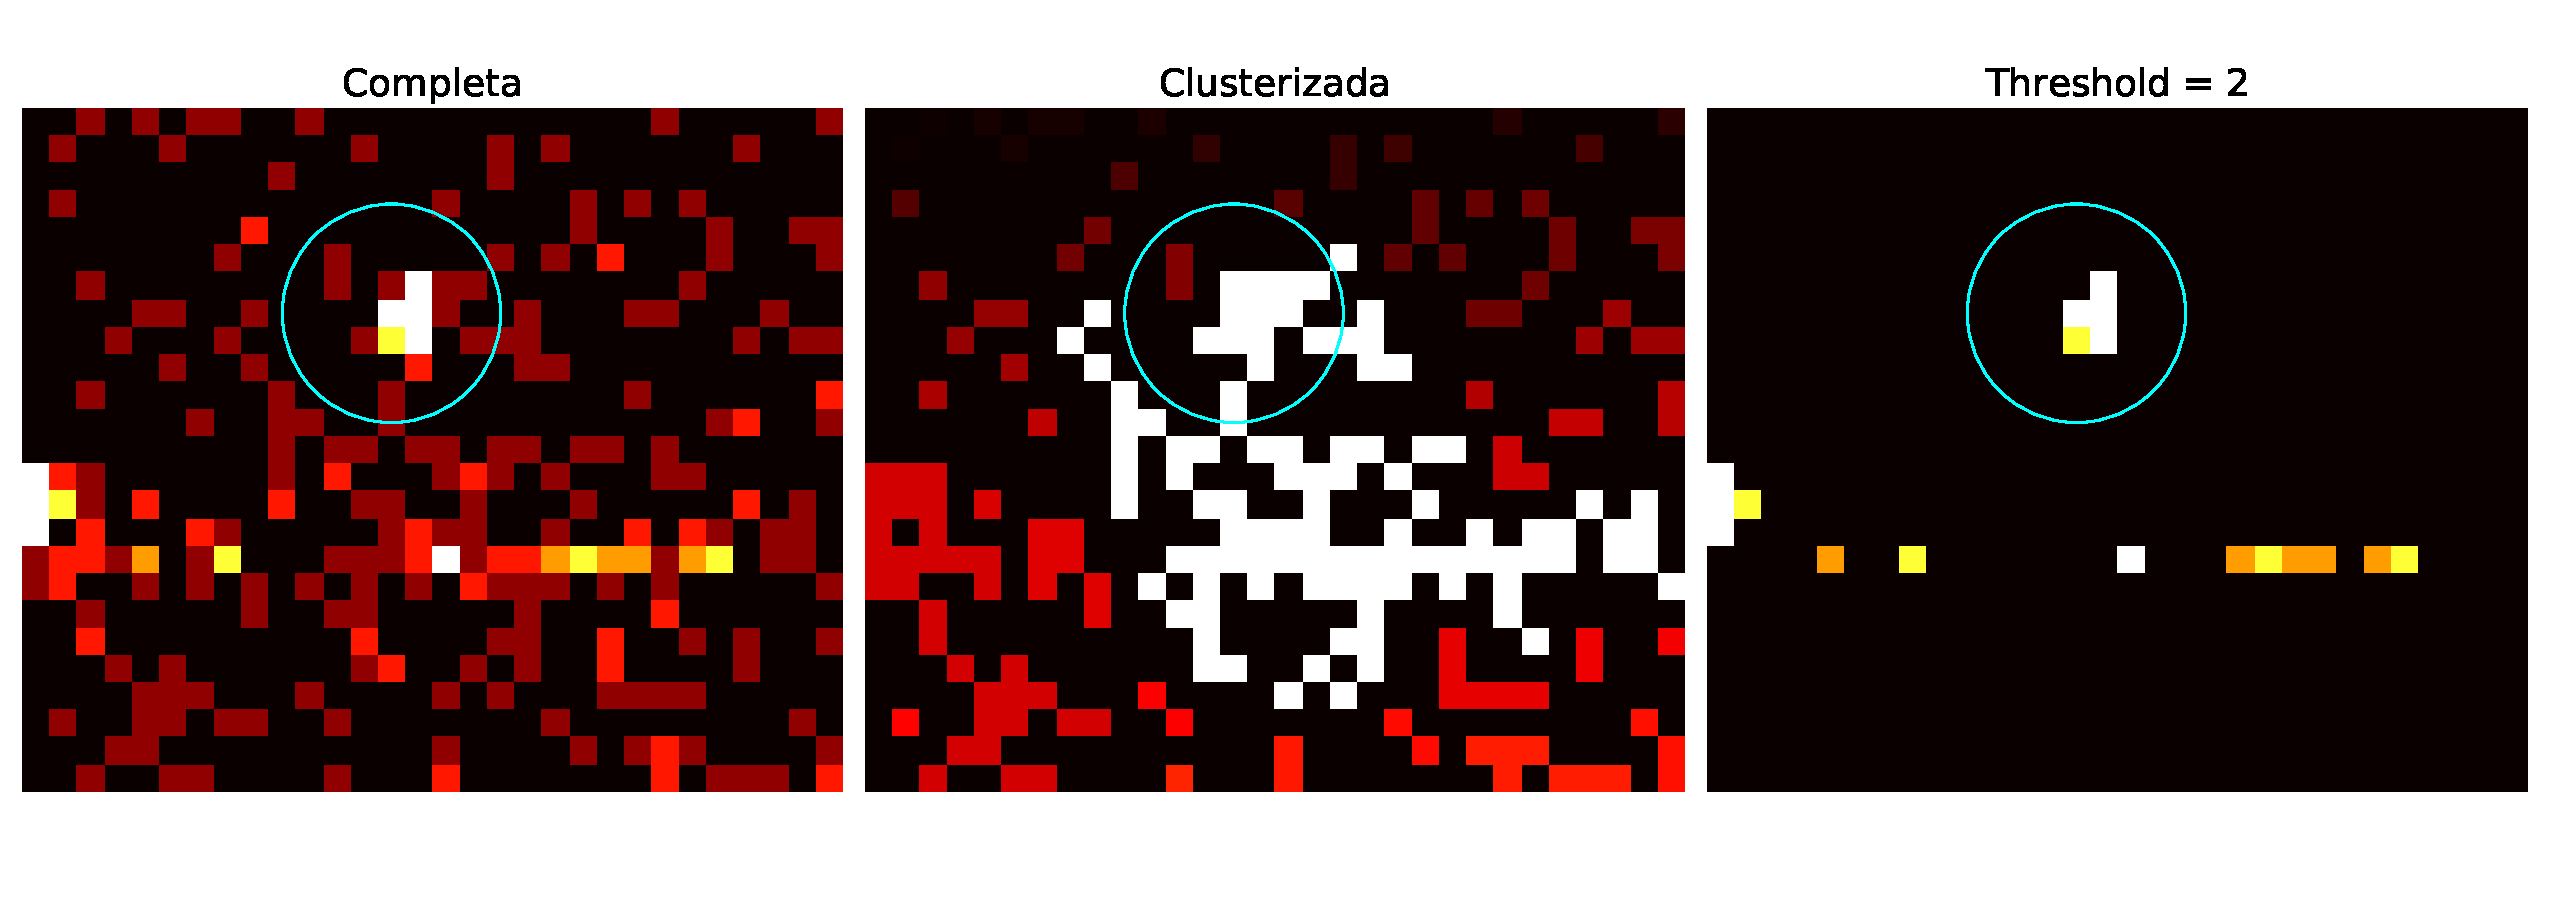
\includegraphics[scale=0.4]{Figs/despegoteo_clusters.pdf}
    \caption{\footnotesize{Ejemplo del caso de un de un evento cercano a los $180$ electrones de carga, que son los eventos de interés. En la imagen de la izquierda se ve la imagen completa, es decir, la medición sin alterar (ya convertida a unidades de carga). En la imagen del centro se ve en blanco y en un degrade muy tenue de rojos los diferentes clusters que el algoritmo logra reconocer. Lo importante de esta imagen es notar que el algoritmo reconoce como un único cluster (blanco) a un número de píxeles muy grande debido justamente a que píxeles con una única carga generan la unión entre todos ellos. Por último, la imagen de la derecha contiene el cluster de interés una vez que los eventos de un electrón son desechados del análisis, haciendo que ahora sí se contabilice correctamente.}}
    \label{fig:ClusterPegoteado}
\end{figure}
De esta forma, se rehicieron los análisis de las imágenes de las mediciones con flúor, con diferentes valores de umbral: \verb|EPIX = 0.5|, \verb|EPIX = 1.5| y \verb|EPIX = 2.5| y se compararon los resultados obtenidos para el conteo total de eventos. Cabe aclarar que estos son resultados preliminares, debido a que la aplicación del umbral añade un sesgo extra al conteo de carga que posteriormente será corregido. Esto se hizo para tres de los cuatro cuadrantes del sensor y para la suma de estos, dado que el segundo cuadrante no funciona correctamente.

%En las Figuras \ref{fig:EntradasVsEpix}, \ref{fig:EnergiadeCreacionVsEpix} y \ref{fig:FanoVsEpix} puede verse la variación de estos parámetros dependiendo del valor de umbral usado. 
%El gráfico más importante en este punto es el de la Figura 
En el gráfico de la Figura \ref{fig:EntradasVsEpix} se observa un drástico aumento en la cantidad de entradas (eventos contabilizados) cuando se varía el \verb|EPIX|. %Se graficaron en cada figura las modificaciones para tres de los cuatro cuadrantes del sensor y para la suma de los cuadrantes $1$, $3$ y $4$. 
%El cuadrante $2$ no funciona correctamente y por eso sus datos no han sido utilizados.
\begin{figure}[h]
%Para hacer estas figs hay que ir a /home/igna/Escritorio/Tesis2021/Figs/pys_para_plots y correr plots_entries_fano_eh.py que usa los datos que están en /home/igna/Escritorio/Tesis2021/Figs/txts_para_plots y se llaman Entries_count.txt
    \centering
    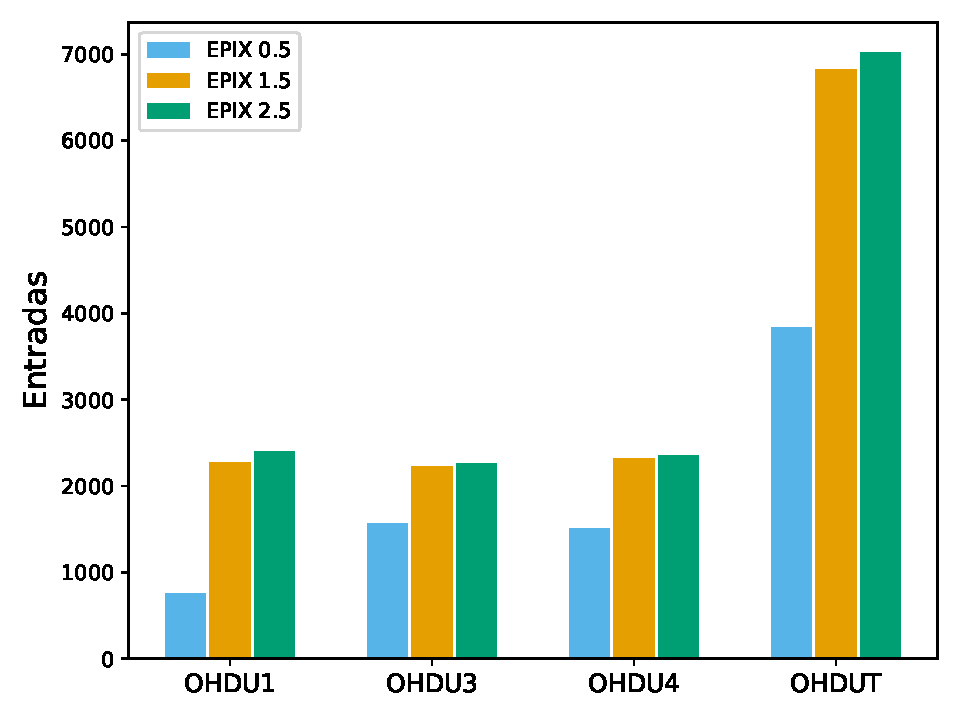
\includegraphics[scale=0.5]{Figs/Entradas_vs_Epix.pdf}
    \caption{\footnotesize{Gráfico de barras para las diferentes cantidad de entradas contabilizadas por el programa, tanto para valores diferentes de EPIX como para los diferentes cuadrantes del sensor. OHDUT hace referencia a la suma de las entradas del resto de los cuadrantes funcionales ($1$, $3$ y $4$). Se observa un aumento de más del doble en la cantidad en la cantidad de entradas para el primer cuadrante, y un aumento importante pero menos pronunciado para el resto de los cuadrantes.}}
    \label{fig:EntradasVsEpix}
\end{figure}
Se puede ver como los cuadrantes $1$, $3$ y $4$ tienen un cambio pronunciado en la cantidad de entradas al pasar de \verb|EPIX = 0.5| a \verb|EPIX = 1.5|, lo cual implica un aumento en la estadística, que era lo que se esperaba, mientras que al pasar de \verb|EPIX = 1.5| a \verb|EPIX = 2.5| el aumento es mucho menos pronunciado. Particularmente, es el primer cuadrante el que registra el mayor incremento en la cantidad de entradas en relación a los otros. En la tabla \ref{tab:EntriesVsEpix} se presentan los valores precisos del cambio en el número de entradas para cada cuadrante para cada valor de \verb|EPIX|. El primer cuadrante pasa de tener $760$ entradas para \verb|EPIX = 0.5| a tener $2272$ para un \verb|EPIX = 1.5|, casi el triple, es un aumento de $\sim 198\%$. En cambio, los cuadrantes $3$ y $4$ pasan de tener $1571$ y $1503$ entradas a $2229$ y $2320$, un aumento muy similar y en torno al $\sim40\%$ y $\sim50\%$ respectivamente.
\begin{table}[h]
\centering
\begin{tabular*}{\textwidth}{c @{\extracolsep{\fill}}ccccc}%{@{}ccccc@{}}
\toprule
           & OHDU 1 & OHDU 3 & OHDU 4 & OHDU 1 + 3 + 4 \\ \hline\hline
EPIX = 0.5 & 760    & 1571   & 1503   & 3834           \\
EPIX = 1.5 & 2272   & 2229   & 2320   & 6821           \\
EPIX = 2.5 & 2399   & 2261   & 2356   & 7016           \\ \bottomrule
\end{tabular*}
\caption{\footnotesize{Diferentes valores para las entradas, para cada uno de los cuadrantes, para los diferentes valores de EPIX utilizados.}}
\label{tab:EntriesVsEpix}
\end{table}
%Efectivamente se observa un aumento en el conteo de eventos que reconoce el programa al aumentar el valor del parámetro \verb|EPIX|. También se observa que el aumento más pronunciado es desde $0.5$ a $1.5$. El aumento promedio en el conteo de eventos es de alrededor del $100\%$.

\begin{comment}
\begin{figure}[h]
%Para hacer estas figs hay que ir a /home/igna/Escritorio/Tesis2021/Figs/pys_para_plots y correr plots_entries_fano_eh.py que usa los datos que están en /home/igna/Escritorio/Tesis2021/Figs/txts_para_plots y se llaman Entries_count.txt
    \centering
    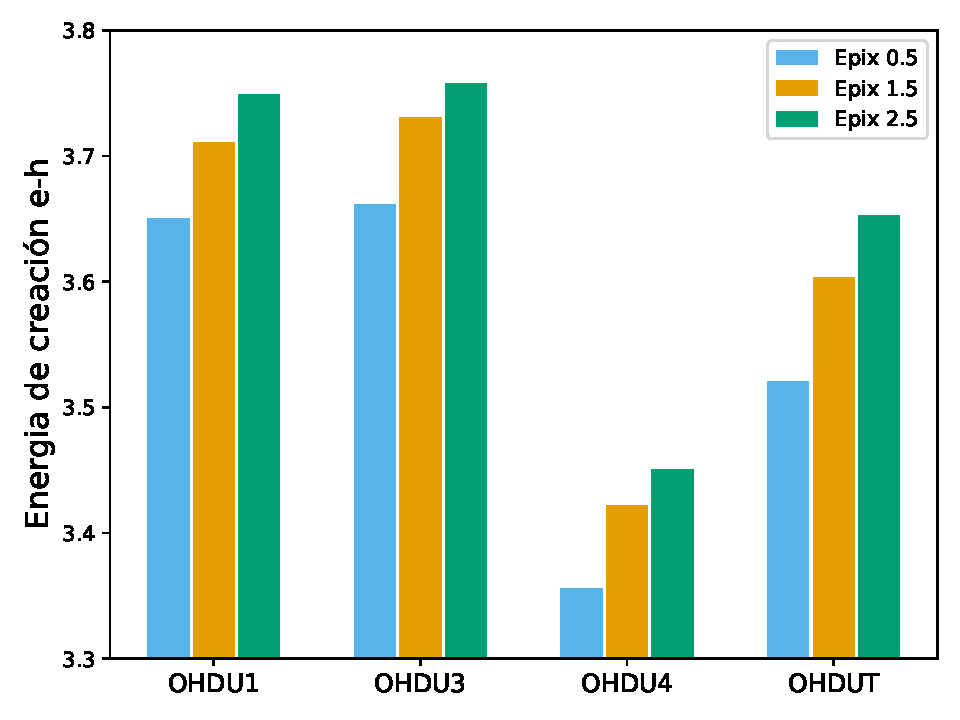
\includegraphics[scale=0.5]{Figs/EnergiaCreacion_vs_Epix.pdf}
    \caption{\footnotesize{Diferentes valores para la energía de creación electrón-hueco en función del EPIX y del cuadrante del sensor utilizado. OHDU hace referencia a al promedio del resto de los cuadrantes funcionales ($1$, $3$ y $4$). Se observa que en todos los casos hay un aumento de la energía de creación electrón hueco cuando aumenta el EPIX.}}
    \label{fig:EnergiadeCreacionVsEpix}
\end{figure}
En cuanto al gráfico de la Figura \ref{fig:EnergiadeCreacionVsEpix}, se ve como el valor preliminar para la energía de creación electrón hueco aumenta en todos los casos al aumentar el umbral \verb|EPIX|. Esto puede deberse al efecto que genera aplicar un umbral y disminuir la carga en los clusters contabilizados, que a su vez son más. Puede suceder que la cantidad de carga en los clusters sufra un corrimiento a la izquierda del valor medio real y por esto la energía de creación electrón-hueco aumente al aumentar el \verb|EPIX|: A un mismo valor de energía, una menor carga ionizada implica una mayor energía de creación electrón-hueco.
Finalmente, el caso más irregular corresponde al gráfico de la Figura \ref{fig:FanoVsEpix}, donde cada cuadrante y para cada valor de \verb|EPIX| el factor de Fano dio valores diferentes y no puede definirse una tendencia a partir de estos resultados. De todas formas es importante recordar que el factor de Fano y la energía de creación electrón hueco obtenidas de estos análisis presentan un sesgo debido a la aplicación del umbral, además del proveniente de eventos de fondo, que debe ser corregido.
\begin{figure}[h]
%Para hacer estas figs hay que ir a /home/igna/Escritorio/Tesis2021/Figs/pys_para_plots y correr plots_entries_fano_eh.py que usa los datos que están en /home/igna/Escritorio/Tesis2021/Figs/txts_para_plots y se llaman Entries_count.txt
    \centering
    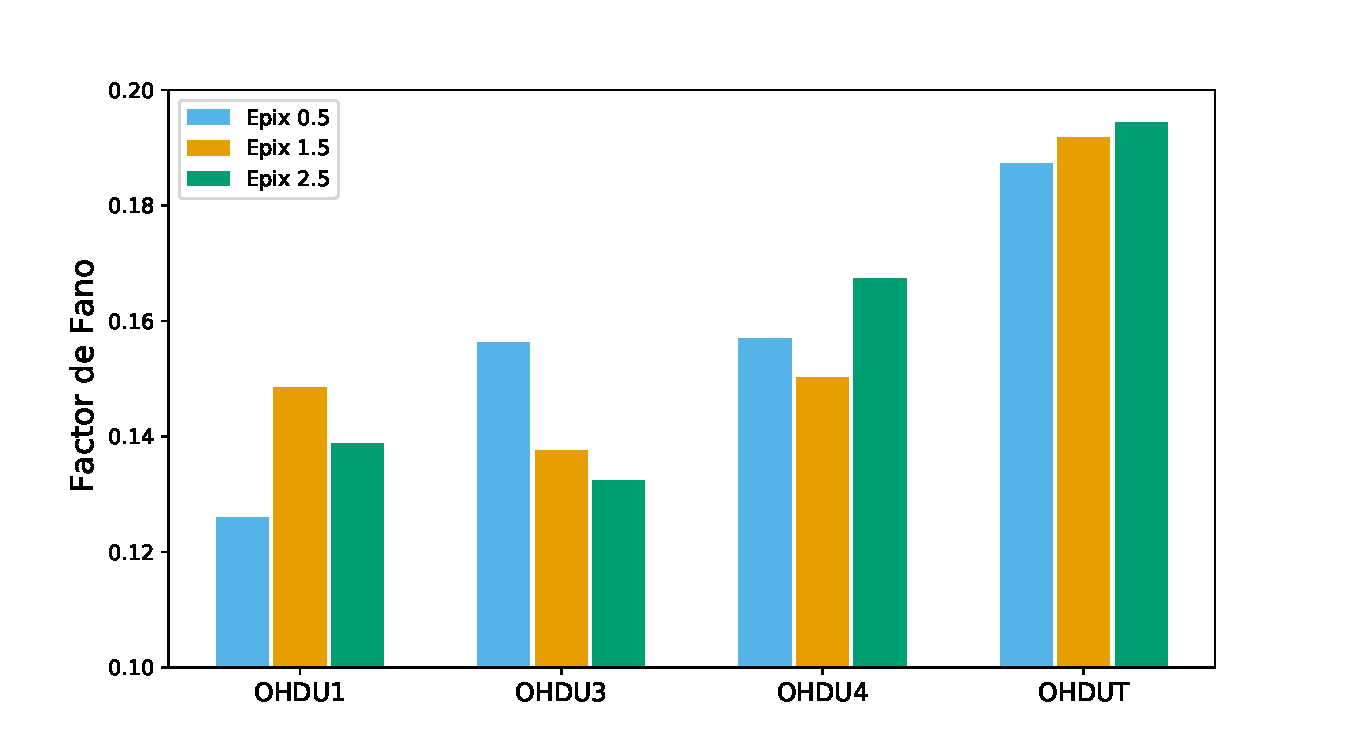
\includegraphics[scale=0.5]{Figs/Fano_vs_Epix.pdf}
    \caption{\footnotesize{Variación del factor de Fano en función del EPIX para diferentes cuadrantes del sensor. No se observa un patrón que se repita.}}
    \label{fig:FanoVsEpix}
\end{figure}
Entonces, del análisis preliminar modificando el umbral de detección de carga por píxel, se puede observar el aumento deseado en la estadística para los eventos de interés de este trabajo. Como se observa que el mayor aumento en la estadística se da para \verb|EPIX = 1.5|, ese es el valor de umbral con el que se realizan los siguientes análisis. No está de más recordar que ese valor de umbral implica desechar los píxeles que tengan menos de $2$ electrones de carga.
\end{comment}
Habiendo tomado este rumbo, es necesario poder remover el sesgo producido por la eliminación de carga en los eventos medidos al aplicar este umbral. Si bien este proceso genera un aumento en la estadística, también genera un corrimiento hacia la izquierda en los picos de interés que debe ser corregido. Además, también es necesario remover el exceso de carga que tengan los clusters de debido al fondo presente en las imágenes y que en este caso genera un corrimiento a la derecha de estos picos. En adelante, la idea es intentar comprender este fondo en las imágenes y con ello poder corregir los valores de carga de los clusters, una vez aplicado el umbral y así mejorar la incerteza de los resultados.

%%%%%%%%%%%%%%%%%%%%%%%%%%%%%%%%%%%%%%%%%%%%%%%%%%%%%%%%%%%%%%%%%%
\section{Caracterización de las imágenes}
\noindent Todo el análisis cuantitativo anteriormente descripto se realizó sin la necesidad de inspeccionar visualmente las imágenes de las cuales se extraen los datos. Simplemente se aplicaron diferentes umbrales de prueba y se contabilizó el aumento en la estadística. Sin embargo, ver las imágenes y rápidamente poder reconocer patrones, como exceso de eventos en una misma región para diferentes imágenes o cualquier característica que visualmente sea reconocible pero que al analizar los datos de forma automatizada pueda quedar ofuscada, es un factor importante a la hora del estudio de los datos. Dado que la cantidad de imágenes utilizadas en este trabajo es superior a las $900$, observar una por una es una tarea monumental e impracticable. Por esta razón fue necesario buscar maneras de poder extraer información contenida en todas las imágenes, de forma práctica y realizable, como por ejemplo, generar una imagen \textit{promedio}. Con este fin, se hizo un análisis visual, cualitativo y cuantitativo de las imágenes para comprender mejor los datos, explorar las características del sensor y de cada uno de sus cuadrantes y poder reconocer posibles deficiencias o particularidades relevantes.

Uno de los primeros factores a caracterizar tiene que ver con la carga de los píxeles que no es debida a eventos de interés. Estos pueden ser producto de corrientes oscuras (electrones que sufren excitaciones espontáneas debido a fluctuaciones térmicas del sensor), rebotes de un haz de baja energía en la cámara donde se encuentra el sensor, etc. No es sencillo y no existe una única manera de estimar el fondo en un sensor, por lo que en este trabajo se ensayaron deferentes maneras de encarar este análisis.

Lo primero que se hizo en este trabajo fue buscar la manera de explorar solamente los píxeles que tuvieran una única carga. Asumiendo que en la gran mayoría de los casos, los píxeles con una única carga que se encuentran aislados de otros píxeles o de clusters de interés, son eventos que forman parte del fondo del sensor, es natural empezar el análisis con estos. Una forma de caracterizar esto es tomar las imágenes y extraer todos los píxeles donde la carga sea mayor que un electrón. De este modo, se obtienen imágenes donde solo hay eventos de un electrón y todo lo demás son píxeles vacíos. En la Figura \ref{fig:ImagenFitsOriginal} se puede ver una típica imagen tomada con el sensor, para el primer cuadrante, en la que claramente pueden observarse algunos eventos muy brillantes y un intenso fondo. En la imagen \ref{fig:ImagenFits1e} en cambio puede verse la imagen resultante de extraer todos los píxeles cuya carga es mayor a un electrón.
\begin{figure}[h]
%Para hacer estas figs hay que ir a /home/igna/Escritorio/Tesis2021/Figs/pys_para_plots y correr imagenes_fits_original_y_filtrada.py
    \centering
    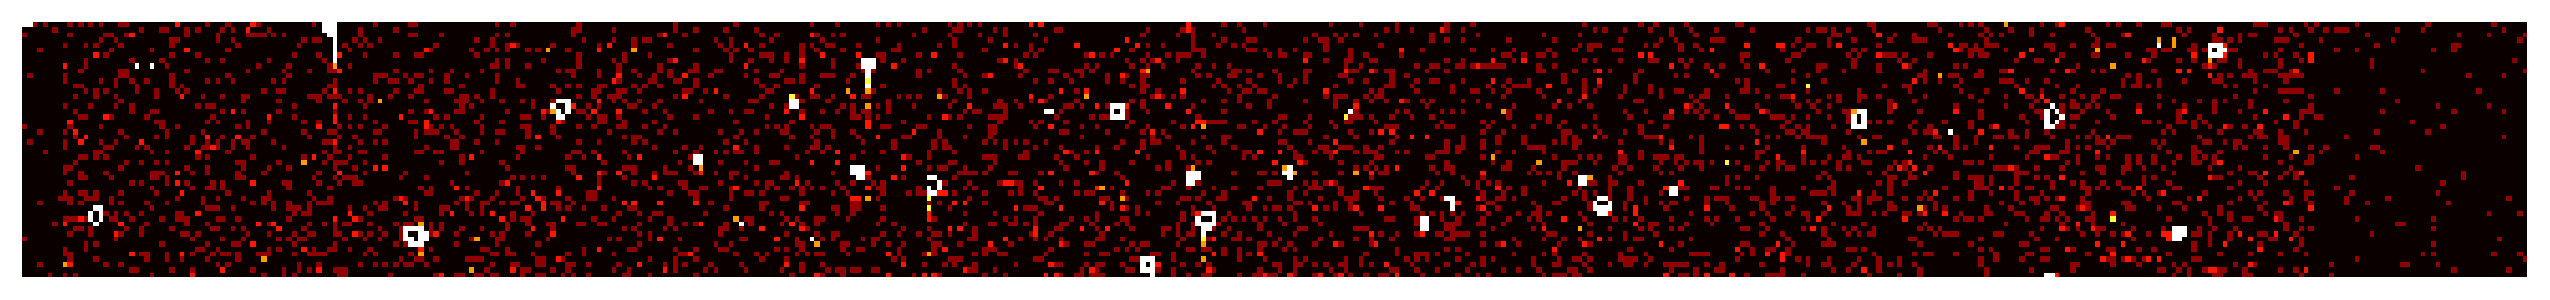
\includegraphics[scale=0.4]{Figs/imagen_fits_original.pdf}
    \caption{\footnotesize{Ejemplo de imagen tomada con el sensor, en el primer cuadrante.}}
    \label{fig:ImagenFitsOriginal}
\end{figure}

\begin{figure}[h]
%Para hacer estas figs hay que ir a /home/igna/Escritorio/Tesis2021/Figs/pys_para_plots y correr imagenes_fits_original_y_filtrada.py
    \centering
    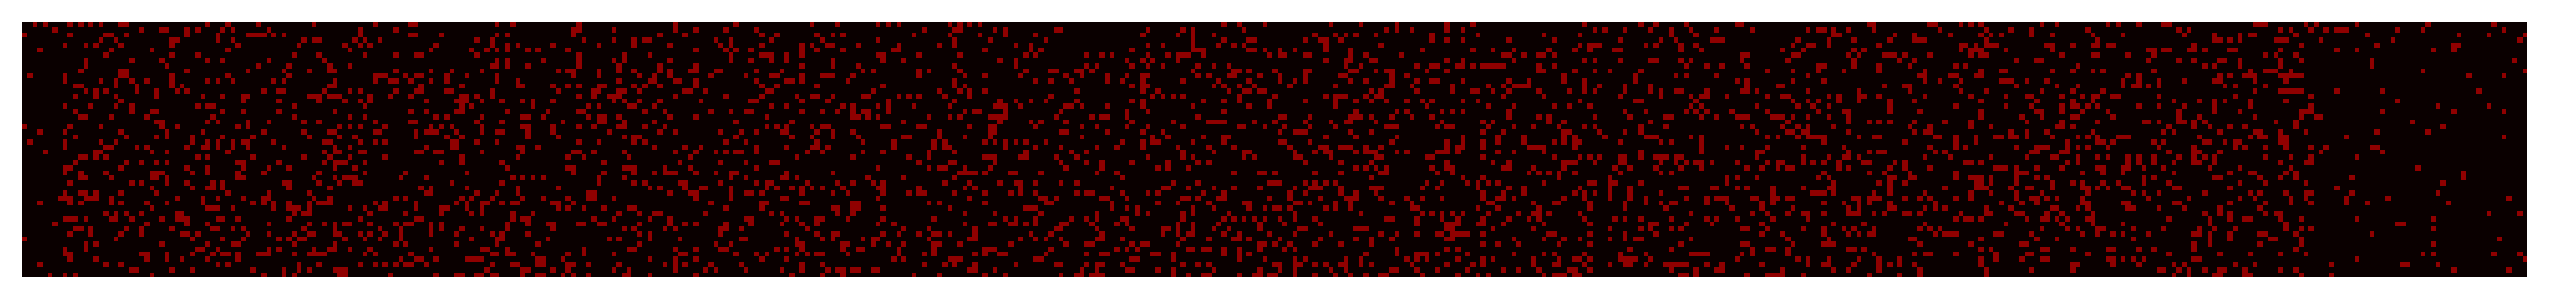
\includegraphics[scale=0.4]{Figs/imagen_fits_1_e.pdf}
    \caption{\footnotesize{Imagen resultante luego de ser extraídos los píxeles con carga mayor a $1$ electrón.}}
    \label{fig:ImagenFits1e}
\end{figure}
Una vez que se extraen los píxeles de carga mayor a uno, se promedian todas las imágenes resultantes y se obtiene una una única imagen que condensa la información de todas las anteriores. En este contexto, promediar las imágenes implica tomar el arreglo matricial con los valores de carga de los píxeles que conforman las imágenes, y realizar la suma convencional de matrices para las más de $900$ imágenes. Finalmente, se divide cada elemento de la matriz suma por la cantidad total de imágenes y se obtiene una imagen donde cada píxel es el promedio de carga de ese píxel para todas las imágenes. De esta forma se puede ver si existen píxeles con mayor o menor tendencia a contener este tipo de eventos.

En la Figura \ref{fig:Eventos1e} se tiene una imagen por cada cuadrante del sensor, promediados en las $\sim 900$ imágenes tomadas, donde los píxeles más brillantes son los que tienen mayor promedio de eventos, es decir, en el total de las imágenes esos píxeles son los que más veces tuvieron un electrón de carga. Esto también puede interpretarse como una imagen de la probabilidad por píxel de que haya un único electrón: Píxeles más brillantes son píxeles más propensos a tener carga.

De la Figura \ref{fig:Eventos1e} pueden destacarse algunas características:
\begin{itemize}
    \item La carga prácticamente nula (en promedio) en las regiones del pre-scan (región izquierda de $7$ columnas de píxeles de extensión) y del over-scan (región derecha de 50 columnas de píxeles de extensión), lo cual es totalmente esperable dado que estas son áreas del sensor que no se encuentran colectando cargas durante la medición. Esto se ve para todos los cuadrantes menos el segundo;
    \item El primer cuadrante es en promedio más brillante que el resto, y se observa un ligero gradiente de intensidad entre las filas inferiores y superiores. Esto se repite, pero en menor medida en los demás cuadrantes pero no necesariamente se observa a simple vista;
    \item El segundo cuadrante (OHDU 2) capta en promedio muy poca carga. Este cuadrante del sensor no funciona correctamente;
    \item En los cuadrantes $3$ y $4$ se pueden ver columnas enteras de píxeles oscurecidas, que captaron muchísima menos carga que podrían deberse a defectos del sensor;
    \item En todos los cuadrantes (menos el segundo), se observa un único píxel (posición $x = 2$, $y = 0$) donde el promedio de carga es mucho mayor al resto. Además, la primera columna de píxeles luego del pre-scan también tiene tendencia a captar más carga que el resto;
    \item Todos los cuadrantes tienen tendencia a tener \textit{hot píxels} en el interior de la región activa, estos son píxeles aislados que tienden a tener más carga que otros. Además pueden verse lineas verticales de \textit{hot píxeles}, llamadas \textit{hot columns} que se producen debido a que un \textit{hot pixel} está generando carga constantemente mientras estas son desplazadas verticalmente durante la lectura.
\end{itemize}
\begin{figure}[h]
%Para reproducir esta figura hay que ir al directorio /home/igna/Escritorio/Tesis2021/Figs/pys_para_plots y correr Skipper_cuadrantes_plot.py
    \centering
    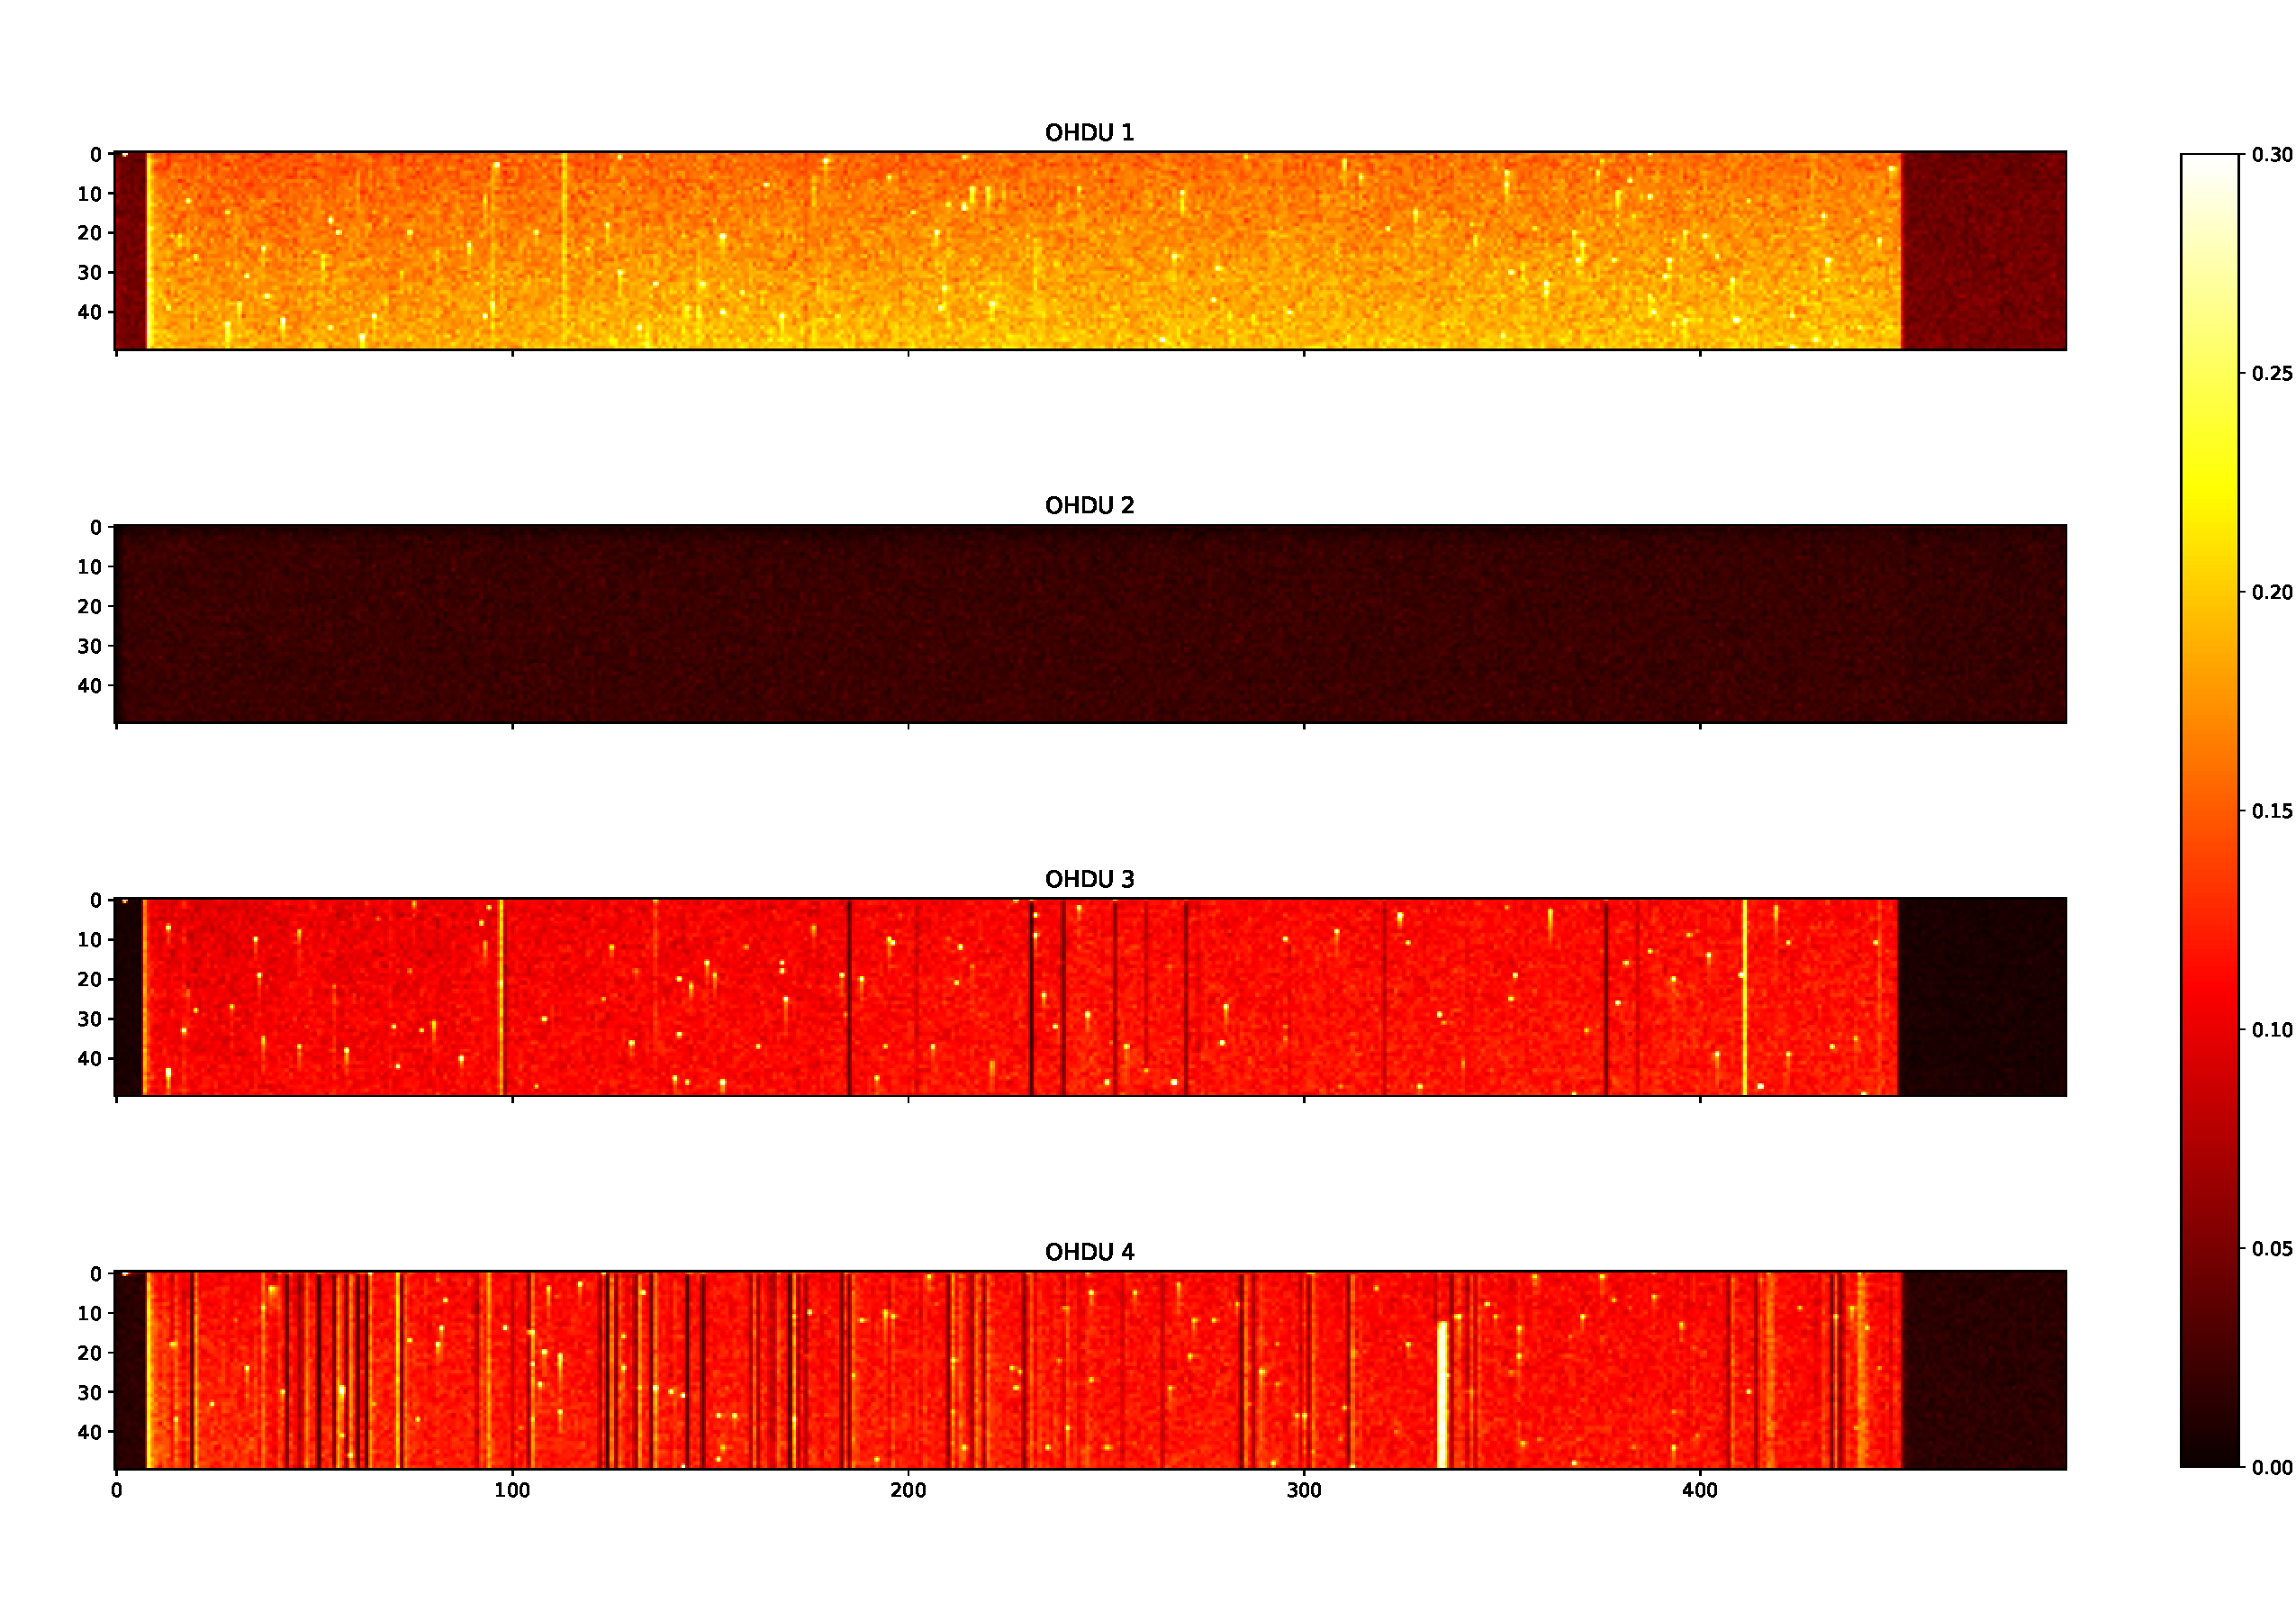
\includegraphics[scale=0.4]{Figs/1ePromedio.pdf}
    \caption{\footnotesize{Imágenes promedio para los $4$ cuadrantes del sensor. Puede verse en la escala de la derecha que los valores más altos que se obtienen rondan el $0.3$, lo cual, interpretado como una probabilidad es un $30\,\%$ de probabilidad de que en ese píxel se encuentre un evento de un electrón. En general se ve que los promedios pueden estar entre $0.1$ y $0.2$ aproximadamente. Es decir, para los cuadrantes funcionales del sensor, cada pixel tiene una probabilidad de tener un único evento que ronda entre el $10\%$ y el $20\%$.}}
    \label{fig:Eventos1e}
\end{figure}
Respecto al gradiente de intensidades que se observa entre filas superiores e inferiores, implicaría una mayor incidencia de eventos de un electrón, en promedio, en los píxeles de las filas inferiores respecto de las filas superiores. Esto puede observarse en los gráficos de Figura \ref{fig:GradienteProb}, donde se ve el aumento en \textit{la probabilidad} media por fila de que haya un evento de un electrón, a medida que el número de la fila aumenta. El gráfico de arriba a la izquierda corresponde al primer cuadrante del sensor, este es el cuadrante donde más evidente se hace este gradiente, además de ser muy lineal. La probabilidad promedio para la fila $0$ del sensor es $\sim 14.5\,\%$ y crece linealmente hasta $\sim 18\,\%$ para la fila $50$. En el gráfico de arriba a la derecha, que corresponde al segundo cuadrante, también se observa un cambio, pero solo entre las primeras 10 filas del sensor, luego la variación de la probabilidad por fila es muy pequeña y parece aproximadamente constante. Además puede verse que los valores son un orden de magnitud menor a los del primer cuadrante. Para los gráficos de abajo a la izquierda y abajo a la derecha, que corresponden a los cuadrantes $3$ y $4$ del sensor respectivamente, se observan también variaciones entre las primeras filas del sensor y las últimas que parecerían tener una tendencia lineal, sin embargo, en comparación a la variación del primer cuadrante, esta es mucho menor. Por esto es difícil verlo a simple vista: la variación para el primer cuadrante es de aproximadamente del $24\,\%$ mientras que la variación de los cuadrantes $3$ y $4$ es aproximadamente del $10\,\%$.

Este gradiente que se observa se debe a que, dado que la medición de carga del sensor es secuencial por filas, las filas superiores son las primeras a las que se les mide la carga, generando que las filas inferiores permanezcan más tiempo expuestas a fuentes de fondo. De todas maneras esta diferencia de tiempo en la lectura de las diferentes filas del sensor es muy pequeña, haciendo que estas diferencias entre filas sea pequeña, aunque apreciable en algunos casos.
\begin{figure}[h]
%Para modificar este plot hay que ir a /home/igna/Escritorio/Tesis2021/Figs/pys_para_plots y correr gradiente_filas_sensor.py Los datos los saca de /home/igna/Escritorio/Tesis2021/Figs/txts_para_plots y del archivo OHDU1/2/3/4_gradiente_filas_sensor.tx
    \centering
    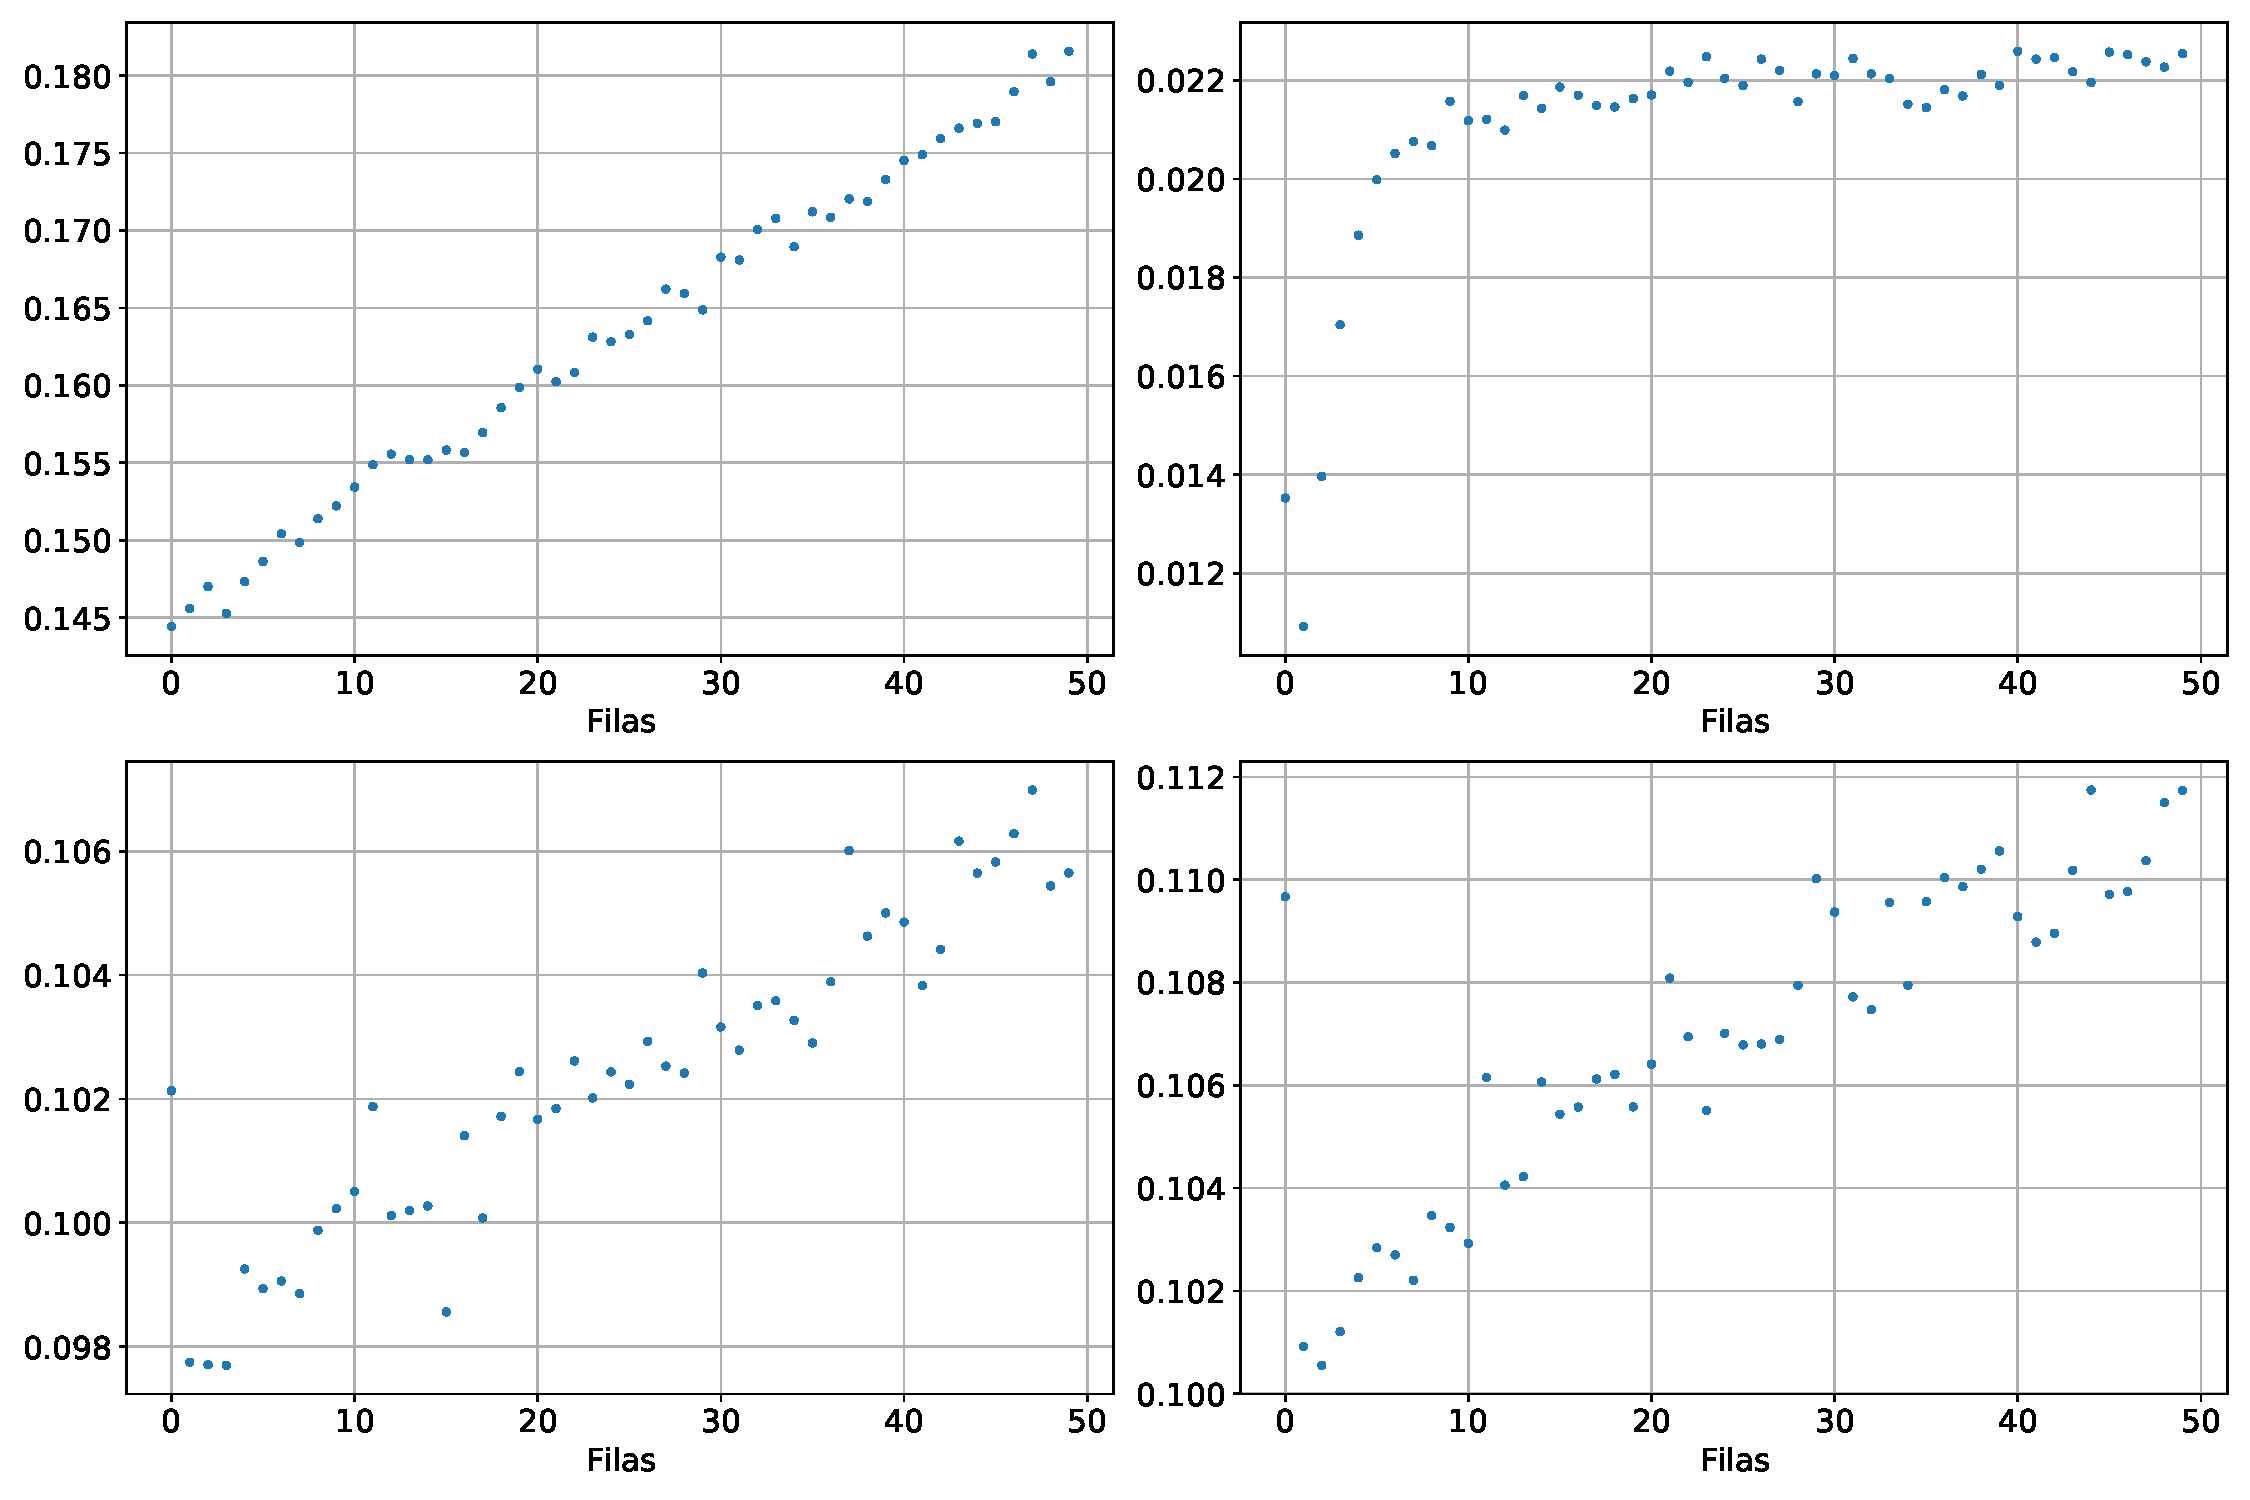
\includegraphics[scale=0.45]{Figs/Gradiente_en_filas_sensor.pdf}
    \caption{\footnotesize{Variación de la \textit{probabilidad} promedio por filas del sensor de tener un evento de $1$ electrón, para los diferentes cuadrantes. Se ven aumentos lineales de la probabilidad para los casos de los cuadrantes $1$, $3$ y $4$ y un aumento más pronunciado en relación a los demás para el primer cuadrante.}}
    \label{fig:GradienteProb}
\end{figure}

Todos los análisis subsiguientes fueron realizados principalmente con el primer cuadrante del sensor, dado que es el cuadrante que mejor funciona.

Teniendo entonces una imagen del promedio de la cantidad de eventos de un electrón por píxel, en la búsqueda por caracterizar el fondo del sensor, lo que se hizo posteriormente fue promediar todos los elementos de esta, de forma de obtener un promedio total y poder interpretarlo como una \textit{probabilidad} general de que en un píxel haya un evento de un electrón. Entonces, para el primer cuadrante y considerando solo la región activa del sensor, se obtuvo una probabilidad $p = 0.1802 \pm 0.0213$, es decir, que con esta primera manera de caracterizar el fondo, hay aproximadamente un $18\,\%$ de probabilidad de que un dado píxel de la región activa del sensor tenga un electrón.

Sin embargo, esta es una forma muy rudimentaria para intentar caracterizar el fondo, además de que no es del todo correcta. Con este camino se asume que todos los eventos de un electrón son fondo, lo cual no es correcto, de forma que la probabilidad de tener un evento de un electrón en un dado píxel, calculada de esta manera, está sobrestimada. Un camino más sofisticado para estimar el ruido en el sensor es explotando el hecho de que los eventos medidos en él siguen una distribución Poissoniana: Si se supone que todo píxel tiene igual probabilidad de tener una carga debido a fondo, que dicha probabilidad es pequeña para mediciones de corto tiempo y que el número de píxeles es muy grande ($22150$ píxeles por cuadrante), entonces es esperable que la distribución que modela estos eventos sea una Poissoniana. De esta forma, si se pudiera calcular la esperanza $\mu$ de la distribución, podría saberse la probabilidad de que en un determinado píxel se encuentre un evento de un electrón o, en general, la cantidad de electrones que se desee.

%%%%%%%%%%%%%%%%%%%%%%%%%%%%%%%%%%%%%%%%%%%%%%%%%%%%%%%%%%%%%%%%%%
\section{Estimación de la esperanza de la distribución}
\noindent Si se considera una distribución Poissoniana para la variable aleatoria \textit{número de electrones de fondo por píxel}, se puede tomar el caso $p = P(k = 1 | \mu) = 0.1802 \pm 0.0213$, que es la probabilidad que se obtuvo previamente. De forma iterativa puede hallarse el valor de $\mu$ que satisface la expresión anterior y resulta ser
\begin{equation*}
    \mu = 0.2258 \pm 0.0276
\end{equation*}
Si bien esta forma de cuantificar el fondo es un poco más general, dado que ahora pueden contemplarse casos más raros, como que un píxel tenga más de una carga, este método sigue teniendo el problema de la sobrestimación de la probabilidad por píxel, al seguir asumiendo que todo píxel con un electrón proviene del fondo.

Siguiendo sobre el mismo camino, todavía bajo la hipótesis de que todo evento de un electrón es debido a fondo, pero evitando el cálculo de los promedios, hay una forma de calcular la esperanza de la distribución y es notando lo siguiente: Si se toman las probabilidades de que haya una sola carga y ninguna carga por píxel, es decir, se toman
\begin{equation*}
    p_{0} \equiv P(k = 0 | \mu),
    \quad
    \quad
    p_{1} \equiv P(k = 1 | \mu)
\end{equation*}
y se mira la relación entre ambas, se tiene
\begin{equation*}
    \frac{p_{1}}{p_{0}} = \frac{\mu\,e^{-\mu}}{e^{-\mu}} = \mu
\end{equation*}
y se observa que puede hallarse directamente el valor de la esperanza de la distribución. Entonces, tomando la región activa de una imagen original (sin separar los eventos de $1$ o más electrones), como la de la Figura \ref{fig:ImagenFitsOriginal}, contando la cantidad de píxeles vacíos, la cantidad de píxeles con $1$ electrón y calculando la relación entre ambas, para todas las imágenes, se puede obtener directamente la esperanza $\mu$ de la distribución. De esto se obtuvo que el valor de la esperanza es:
\begin{equation*}
    \mu = 0.2311 \pm 0.0001
\end{equation*}
Los resultados de ambos métodos difieren en menos del $5\,\%$ y se solapan sus errores. Si bien esta segunda forma para calcular la esperanza $\mu$ parece un poco más elegante y correcta, el problema sigue estando en los datos que se utilizan para calcularla. El valor seguirá estando sobrestimando respecto del valor real, en tanto se siga considerando a todo píxel con un único electrón como fondo.

No hay que perder de vista que el objetivo de calcular la esperanza de la distribución es poder utilizarla para estimar cuánta carga extra hay sobre los clusters debida a fondo y cuánta carga no espuria fue removida debido al umbral aplicado. Conociendo la esperanza de la distribución de eventos de fondo y la cantidad de píxeles que ocupa un cluster, puede calcularse la cantidad esperada de carga extra que se halla en cada cluster. Teniendo estos valores, puede corregirse el valor de la carga y con eso hacer mejores estimaciones del factor de Fano y la energía de creación electrón-hueco.

Pero también, para poder generar una corrección en el conteo de cargas por cluster y que esté lo menos sesgada posible, hay que tener en cuenta las posibles formas en las que un cluster podría tener más o menos carga:
\begin{itemize}
    \item Que sobre la superficie de los clusters hayan eventos de más debido a fondo;
    \item Dado que en este análisis se está aplicando un umbral que elimina eventos de menos de dos electrones, podría suceder que a un cluster se le quiten eventos reales que se encuentran en sus bordes.
\end{itemize}
Con lo cual no solo es necesario corregir la carga por exceso en los clusters, sino también por defecto. Por ello, la esperanza que se obtuvo de calcular la relación entre eventos de un electrón y píxeles vacíos contiene tanto información de eventos espurios como información de eventos genuinos. Pero lo que se persigue es poder identificar los eventos espurios y los genuinos por separado. En ese sentido puede decirse que 
\begin{equation*}
    \mu_{T} = \mu_{bkg} + \mu_{g}
\end{equation*}
donde $\mu_{bkg}$ es la esperanza de la distribución de la variable aleatoria \textit{cantidad de eventos espurios por píxel}, mientras que $\mu_{g}$ es la esperanza de la variable aleatoria \textit{cantidad de eventos genuinos por píxel}. Hay que lograr separar ambos efectos para poder aplicar las correcciones correctamente. Queda claro que hasta el momento solo se calculó $\mu_{T}$, sin poder discriminar ambas contribuciones. La forma en la que se llevó a cabo la separación entre ellas se detalla a continuación.

%%%%%%%%%%%%%%%%%%%%%%%%%%%%%%%%%%%%%%%%%%%%%%%%%%%%%%%%%%%%%%%%%%
\subsection{Cálculo de las contribuciones al valor medio total}
\noindent Hasta el momento, ambos métodos utilizados para calcular $\mu_{T}$ consistían en analizar los eventos de un electrón en toda el área activa del sensor. Sin embargo, esto traía aparejada una sobre estimación en los cálculos dado que se asumió que todo evento de un electrón era fondo, lo cual no es cierto. Por otro lado, considerando que la distribución de eventos por píxel tiene tanto contribuciones de fondo como genuinas, es necesario poder separar ambas contribuciones y no existe forma de hacerlo al estudiar toda el área activa del sensor.

Para poder separar ambas contribuciones al calcular el $\mu_{T}$, se puede restringir el análisis al entorno cercado de los clusters, donde ahora por clusters se entiende todo píxel individual de dos o más electrones de carga, o conjunto de píxeles donde cada uno tenga como mínimo dos electrones de carga. Es decir, se toma una imagen que tiene eventos de dos o más electrones, y los demás eventos se hacen cero. En la imagen de la Figura \ref{fig:ImagenFits2omasElectrones} se puede ver como se ve una imagen de estas características.
\begin{figure}[h]
%Para modificar este plot hay que ir a /home/igna/Escritorio/Tesis2021/Figs/pys_para_plots y correr imagen_fit_2_o_mas_e.py
    \centering
    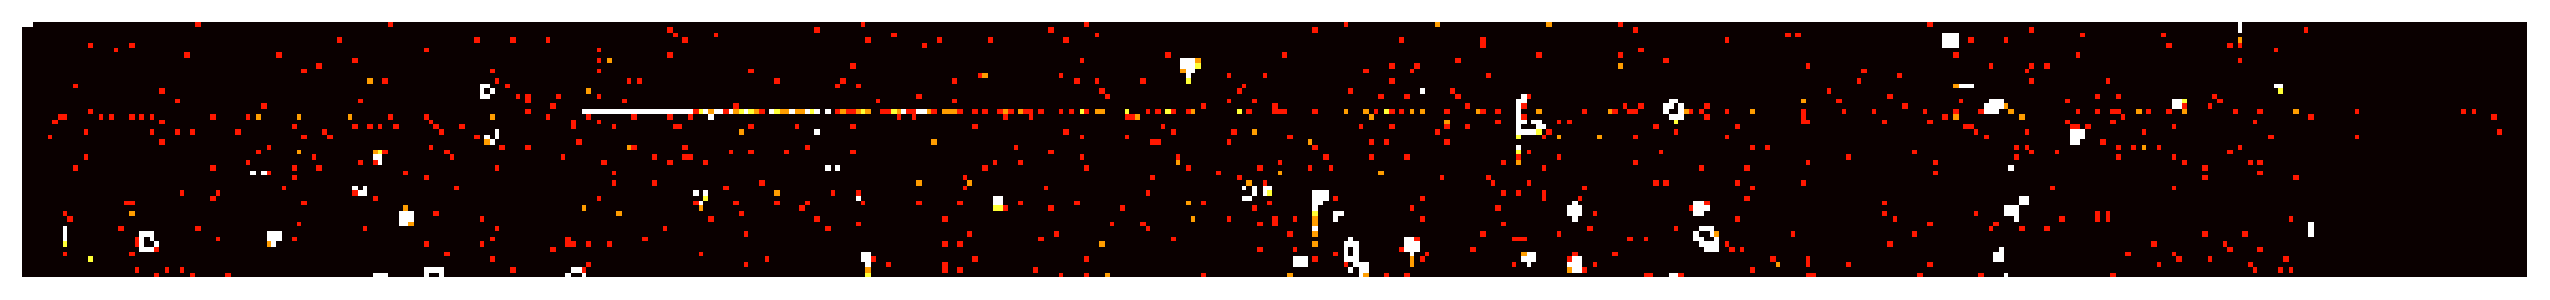
\includegraphics[scale=0.4]{Figs/imagen_fits_2_o_mas.pdf}
    \caption{\footnotesize{Imagen de ejemplo en la que solo hay píxeles que tengan dos o más electrones.}}
    \label{fig:ImagenFits2omasElectrones}
\end{figure}
En el entorno cercano de los clusters, más precisamente, en los píxeles inmediatamente contiguos a los píxeles con carga, a partir de ahora  \textit{primer borde}, es la región donde se puede decir con seguridad que coexisten ambas contribuciones: fondo y eventos genuinos. En cambio, la región formada por los píxeles que se encuentran separados por un píxel entre ellos y los eventos, a partir de ahora \textit{segundo borde}, es la región donde la probabilidad de que haya eventos de un electrón que sean genuinos y que por difusión terminaron alejados de su cluster es tan baja que puede considerarse nula. Con lo cual, en esta región y toda región más lejana a los clusters puede considerarse que los eventos de un electrón que se encuentren solo pueden deberse a fondo.

Sabiendo que existe una región donde se encuentran ambas contribuciones juntas y otra región donde solo se puede encontrar la contribución de fondo se pueden calcular y obtener todas las contribuciones por separado.

El método utilizado consistió en tomar el primer borde de los clusters para calcular allí el valor de $\mu_{T}$. El procedimiento se basó en formar una máscara del primer borde de los clusters. Para eso se tomaron todos los eventos de dos o más electrones y se los expandió un píxel en todas las direcciones para formar la primera etapa de la máscara. Luego, se vacío el interior de esta dejando solo sus contornos, que coinciden con los píxeles contiguos a los bordes de los clusters. Luego, superponiendo la máscara sobre la imagen original (ahora con todos los eventos), se cuentan los píxeles con eventos de un electrón y los píxeles vacíos cayeron sobre la máscara. 
\begin{figure}[H]
%Para modificar este plot hay que ir a /home/igna/Escritorio/Tesis2021/Figs/pys_para_plots y correr imagen_bordes2.py
    \centering
    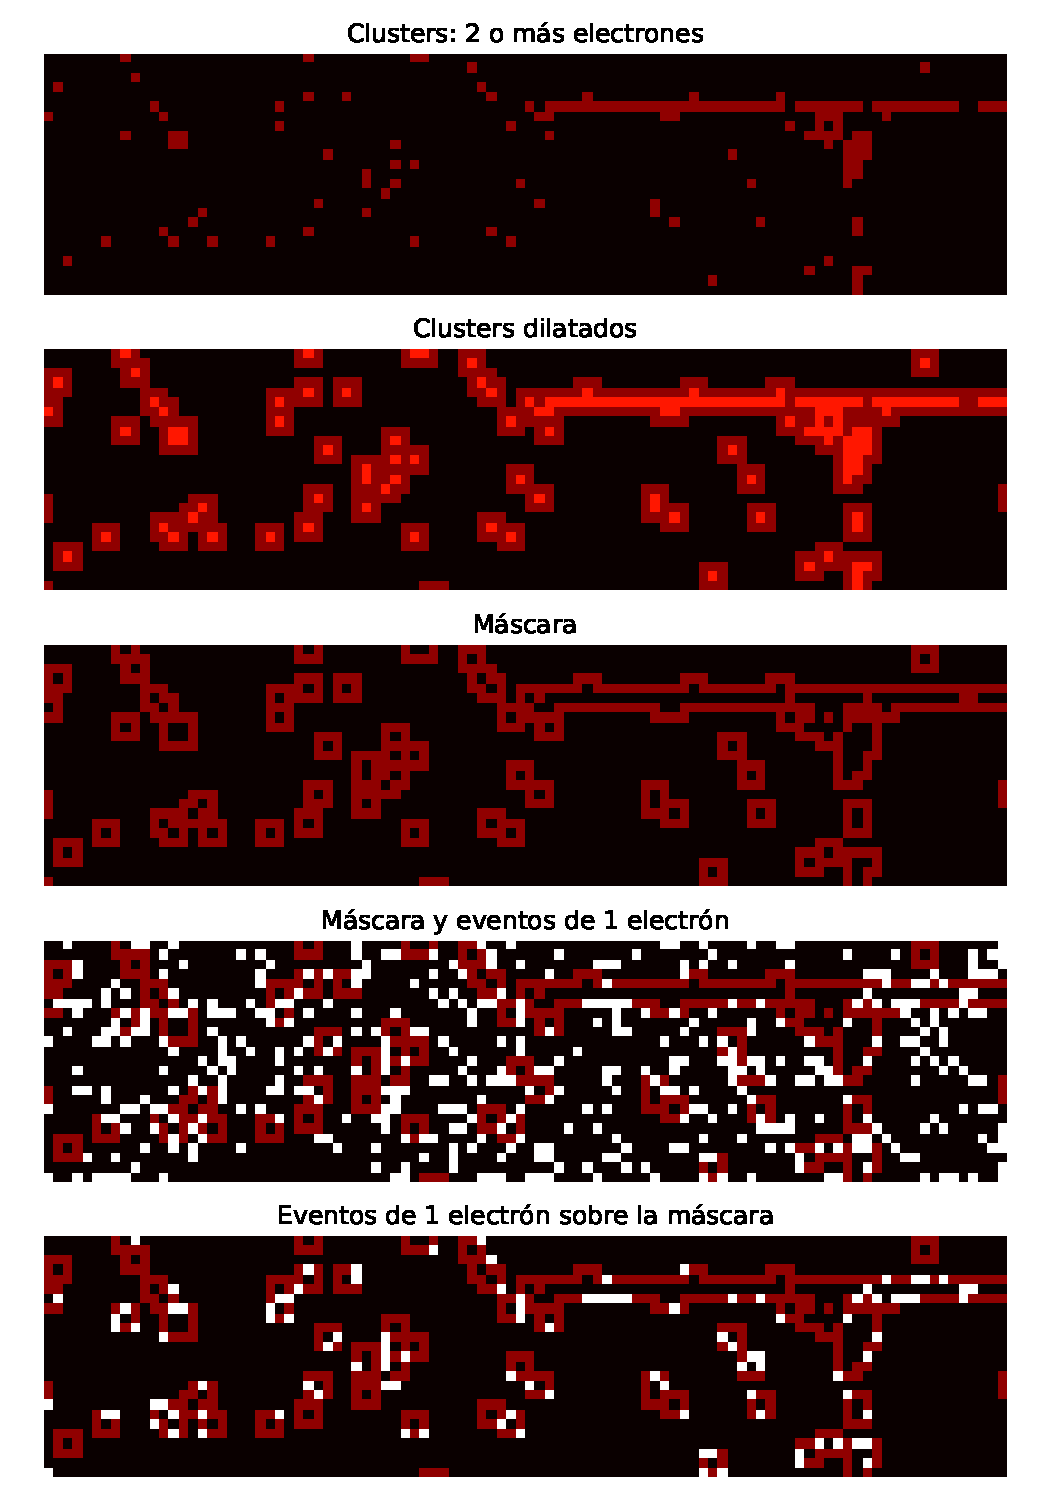
\includegraphics[scale=0.7]{Figs/analisis_bordes.pdf}
    \caption{\footnotesize{Diferentes partes del proceso de análisis de los bordes de los clusters para una imagen de ejemplo. En cada figura se ve una porción de $25 \times 100$ píxeles de área. En la primera imagen (de arriba a abajo) se tienen los clusters de dos o más electrones. En la segunda imagen se representa la dilatación de los clusters aumentando en un píxel en todas las direcciones. En la tercera imagen se ve la diferencia entre las dos primeras imágenes y se la define como la máscara a utilizar. En la cuarta se ve la máscara y superpuestos todos los eventos de un electrón de esa porción del sensor. Finalmente, en la quinta se ven solo los eventos de un electrón que cayeron encima de los píxeles de máscara. Son estos eventos los que son se cuentan en todas las imágenes, junto con los píxeles vacíos de la máscara para calcular el $\mu_{T}$.}}
    \label{fig:AnalisisBordes}
\end{figure}
Nuevamente, calculando la relación entre eventos de un electrón y píxeles vacíos, se obtiene $\mu_{T} = 0.2049 \pm 0.0002$, dado que en el primer borde se encuentran las dos contribuciones. En la Figura \ref{fig:AnalisisBordes} puede verse gráficamente cada uno de los pasos que se llevó a cabo para generar la máscara y contabilizar los eventos de un electrón que se solapan con ella.

Conociendo el valor de $\mu_{T}$, resta obtener la contribución del fondo que da origen a $\mu_{bkg}$. En primer lugar se ensayó utilizar la región conformada por el segundo borde y los píxeles aún más lejanos para calcular el $\mu_{bkg}$, es decir, toda la región restante del sensor donde hay eventos espurios. Para esto, utilizando la máscara previamente obtenida, en vez de observar los eventos de un electrón de la imagen original que solapan con ella, se cuentan con eventos de un electrón y los vacíos que están fuera de ella. De calcular la relación entre ambos, como se hizo previamente, se obtiene que el valor para el valor medio de la contribución del fondo es $\mu_{bkg} = 0.1621 \pm 0.0001$. 

Sin embargo, esta forma de calcular el fondo puede mejorarse un poco más. El objetivo del cálculo de estos valores medios es poder utilizarlos para corregir la carga medida en los clusters, debido al fondo y al umbral utilizado. Es por eso que los valores de las contribuciones que se están buscando deben ser las más representativas de los sesgos que los eventos existentes en los eventos de interés. En ese sentido, puede resultar que los eventos de fondo que se encuentran lejos de los eventos de interés no sean los más representativos de los eventos de fondo que producen un sesgo en ellos, con lo cual se estaría obteniendo una corrección debido a fondo que no influye sobre el conteo de carga final. Con lo cual, para calcular un valor de $\mu_{bkg}$ más representativo a los clusters, se optó por solo mirar el segundo borde y no todo el resto del sensor.

El procedimiento es el mismo que para el primer borde, pero ahora expandiendo los clusters en dos píxeles en todas las direcciones, y quedándose únicamente con el segundo borde, donde no hay píxeles con carga genuina y donde se tienen los eventos de fondo más representativos para los clusters. Este proceso puede verse en la imagen \ref{fig:AnalisisBordesx2}. Nuevamente, de la relación entre los eventos de un electrón y los píxeles vacíos que se solapan con la máscara, se obtiene $\mu_{bkg} = 0.1902 \pm 0.002$. Finalmente, teniendo el valor de $\mu_{T}$ y el valor de $\mu_{bkg}$ queda completamente determinado el valor de $\mu_{g}$.
\begin{figure}[h]
%Para modificar este plot hay que ir a /home/igna/Escritorio/Tesis2021/Figs/pys_para_plots y correr imagen_bordesx2.py
    \centering
    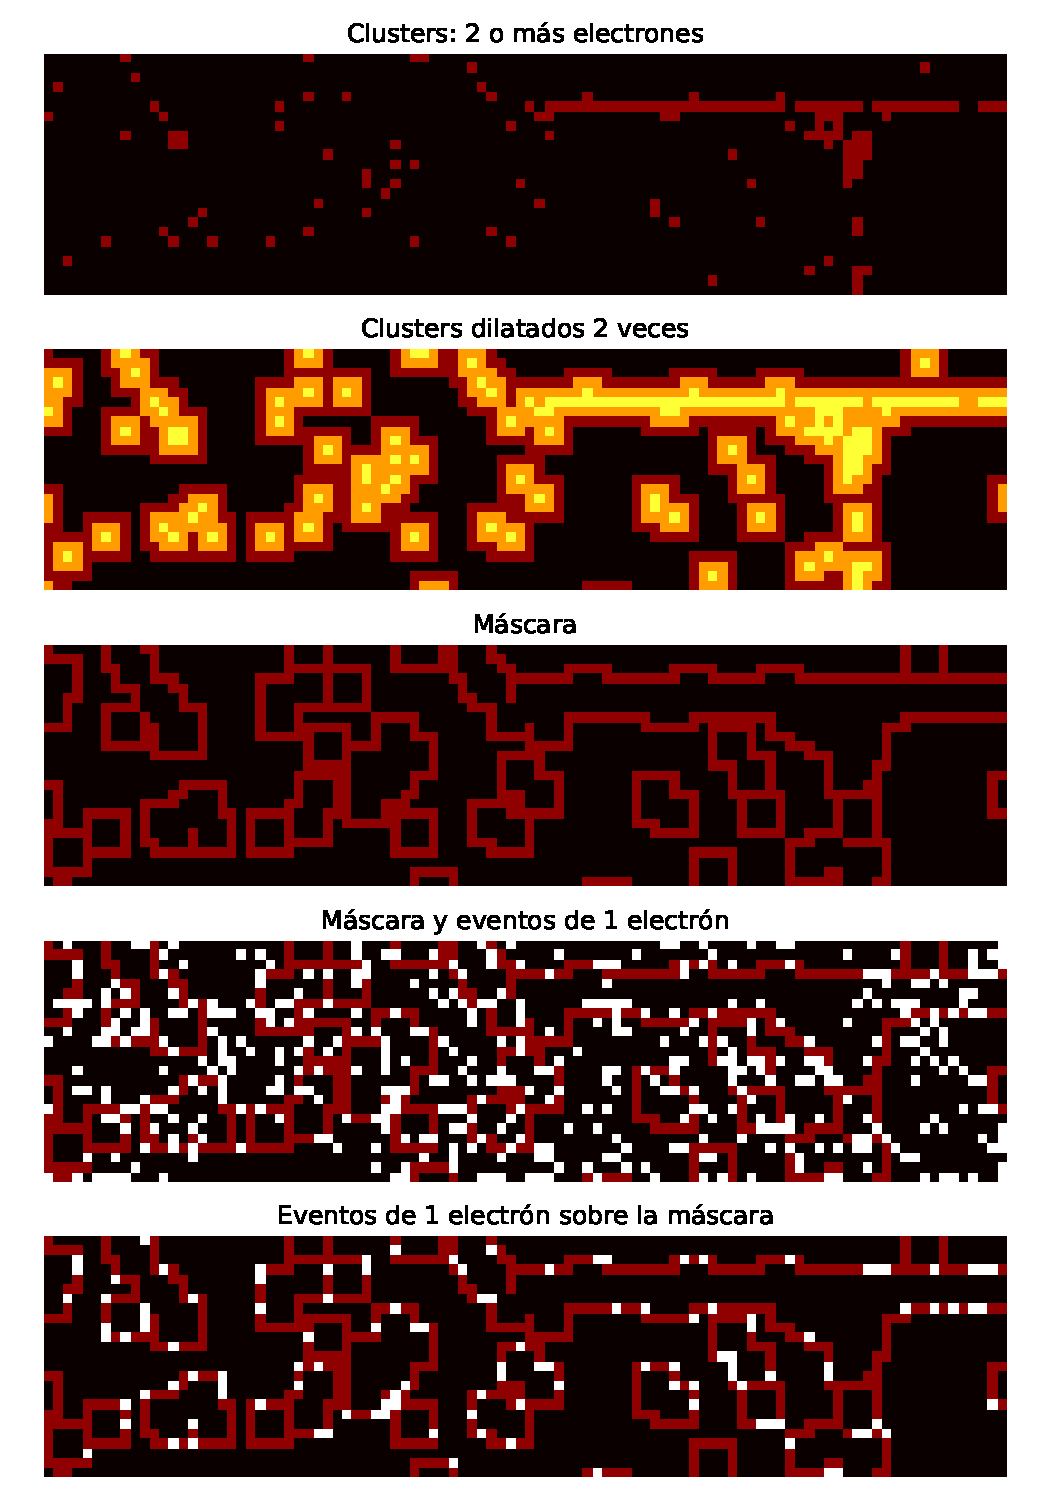
\includegraphics[scale=0.7]{Figs/analisis_bordesx2.pdf}
    \caption{\footnotesize{Análoga a la Figura \ref{fig:AnalisisBordes}, pero para el caso de $2$ dilataciones, de forma de generar una máscara en el segundo borde. Los pasos son los mismos antes descriptos. De este proceso se halla la esperanza $\mu_{bkg}$.}}
    \label{fig:AnalisisBordesx2}
\end{figure}
De realizar estos análisis se obtuvieron los valores para las esperanzas de ambas contribuciones, calculadas sobre el conjunto de más de $900$ imágenes provenientes de mediciones de los rayos $X$ del flúor y para el primer cuadrante del sensor, que resultaron ser:
\begin{equation*}
    \mu_{T} = 0.2040 \pm 0.0002
\end{equation*}
y el valor de la esperanza para los eventos espurios resultó 
\begin{equation*}
    \mu_{bkg} = 0.1961 \pm 0.0002
\end{equation*}
con lo cual, la esperanza para los eventos genuinos es 
\begin{equation*}
    \mu_{g} = 0.0079 \pm 0.0003   
\end{equation*}

%%%%%%%%%%%%%%%%%%%%%%%%%%%%%%%%%%%%%%%%%%%%%%%%%%%%%%%%%%%%%%%%%%
\subsection{Corrección del conteo de carga}
\noindent El punto del análisis anterior era generar las herramientas para corregir el conteo de carga que hace el programa de reconstrucción de eventos luego de aplicar el umbral que elimina todos los eventos menores a dos electrones

Esta corrección se llevó a cabo modificando el código del programa que es usado por \textit{ROOT} para calcular el factor de Fano, la energía de creación electrón-hueco, y otras variables, por medio del ajuste no bineado de los espectros de carga. Los espectros son reconstruidos utilizando la información de los clusters que está contenida en el archivo \verb|.root| generado por \verb|skExtract.exe| al procesar las imágenes, como se describió en la Sección \ref{sec:ProcesadoDatos}. Al contar la carga de estos clusters y conociendo el área de los mismos (cantidad de píxeles que los conforman), se agrega y se quita carga en función de los valores hallados antes.

Dado que la cantidad de carga por píxel sigue una distribución poissoniana, de esperanza $\mu$, para cada tipo evento (espurio, genuino o total) se tiene una esperanza. Para calcular la cantidad de carga que se espera que tenga un cluster de $N$ píxeles en el sensor, se puede hacer uso de las propiedades de la esperanza. Sea $Y = \sum\limits_{i = 1}^{N} X_{i}$, donde $X_{i}$ son distintas realizaciones de la variable aleatoria con distribución Poissoniana y $N$ es el número de píxeles del cluster, entonces la esperanza de la nueva variable aleatoria $Y$ se calcula como
\begin{equation*}
     E(Y) = 
     E
     \left(
         \sum\limits_{i=1}^{N} X_{i}
     \right)
     = \sum\limits_{i=1}^{N}E(X_{i})
     = \sum\limits_{i=1}^{N}\mu_{i}
\end{equation*}
pero como $X_{i}$ son distintas realizaciones de la misma variable aleatoria, entonces tienen todas la misma esperanza, es decir $\mu_{i} = \mu\ \forall\ i$, con lo cual
\begin{equation*}
    E(Y) = N\mu
\end{equation*}
con lo cual, la cantidad de carga esperada para un cluster viene dada por el producto entre la esperanza de la distribución y la cantidad de píxeles del cluster. De esta forma, sabiendo que la esperanza se puede escribir como $\mu_{T} = \mu_{bgk} + \mu_{g}$, las correcciones se pueden realizar aplicando esta misma receta a los valores de carga por cluster. Si $n_{e}$ es la cantidad de carga medida en un dado cluster, la corrección de este valor de carga será $n_{c}$ y viene dado por
\begin{equation*}
    n_{c} = n_{e} + N(\mu_{g} - \mu_{bkg})
\end{equation*}
es decir, se agrega la cantidad de carga que se estima se pierde en los bordes por aplicar el umbral \verb|EPIX = 1.5| y se quita la carga estimada de fondo en el interior de los clusters. En la práctica este procedimiento es simplemente agregar una línea en el código, justo después de la medición de carga de un cluster, donde se actualiza el valor de carga con la expresión anterior.

El metodo descripto se utilizará para corregir el sesgo introducido al cambiar \verb|EPIX| y el preexistente por el fondo. Los resultados finales se presentan en el Capítulo \ref{chap:Resultados}.